\section{Vehicle Description}
\label{sec:Vehicledescription}
The technology which has been provided for the prototype is a tracked vehicle, seen on \figref{TrackedVehicle}. A platform as the same size of the vehicle is mounted on the vehicle to protect the mechanical system and to support the system, which includes PCB boards, the battery, and the sensors used to control the vehicle. When the platform is mounted on, the vehicle is 45 cm long, 29 cm in width, 12 cm in height and it weighs 2932 grams.\\
%
\begin{figure}[H]
	\centering
	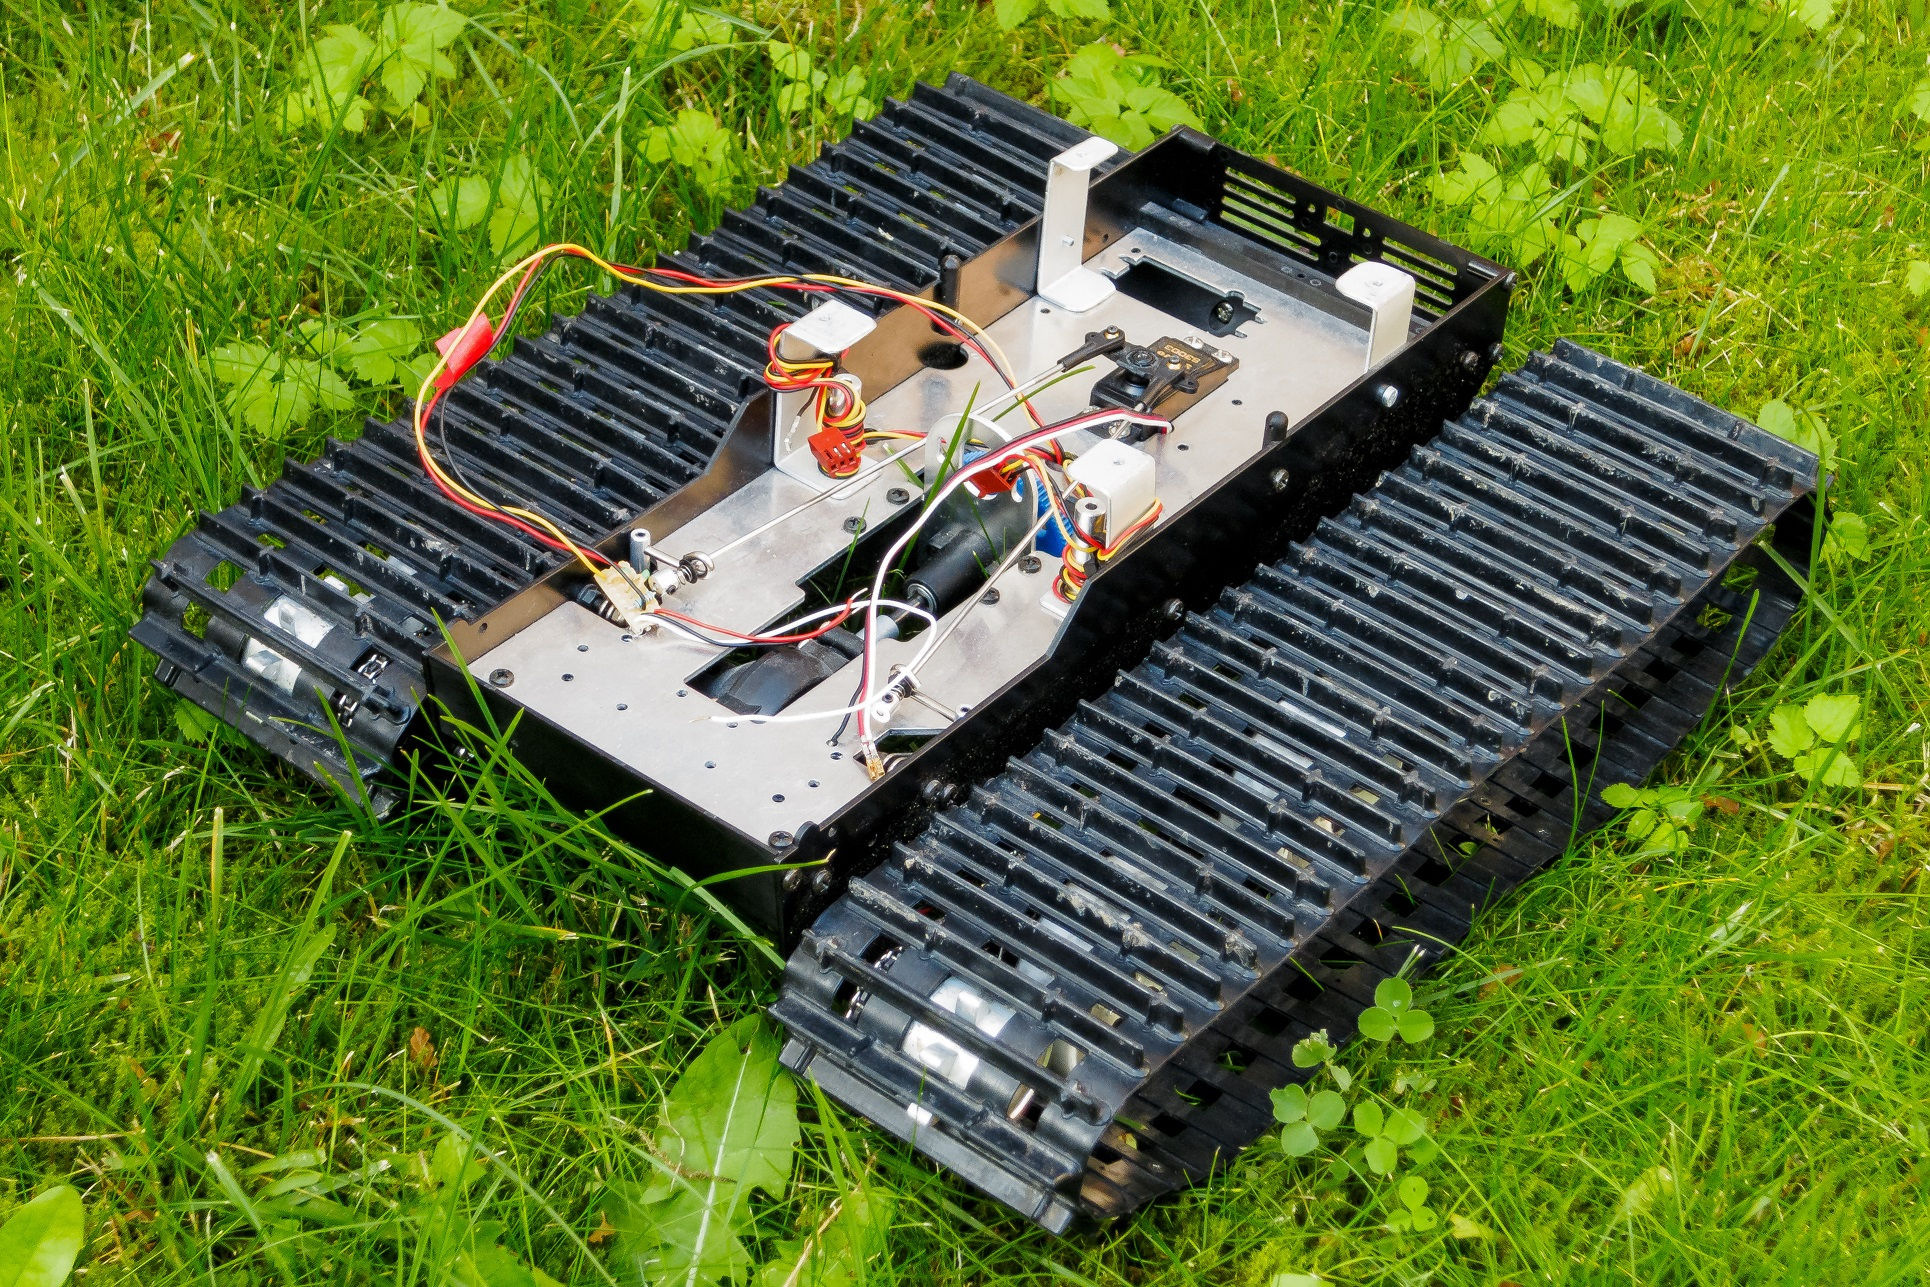
\includegraphics[scale=0.6]{figures/BeltVehicle.jpg}
	\caption{The provided tracked vehicle}
	\label{TrackedVehicle}
\end{figure}
%
To get an understanding of how the motor is used to make the belts rotate one must comprehend how the drivetrain functions. To make the vehicle turn it is necessary to understand how the servo acts on the breaks connected to the driving wheels in either side. Hall sensor are attached by the provided vehicle's drive gears on either side, along with 4 magnets attached to either drive gear. To run the vehicle a rechargeable battery pack is also provided.